\documentclass{standalone}
\usepackage{tikz}

\usetikzlibrary{decorations.pathreplacing}

\begin{document}

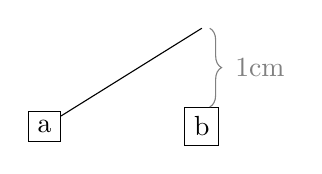
\begin{tikzpicture}
%x description="shift a single coordinate"

\node[draw] (a) at (0,0) {a};
\node[draw] (b) at (2,0) {b};

%x step={
\draw (a) -- 
% option inside coordinate parenthesis
	([yshift=1cm] b.north);
%x }
	

\draw [decorate, decoration={brace, amplitude=0.15cm}, gray]
	([yshift=1cm, xshift=0.1cm] b.north) 
	-- node [right=0.2cm] {1cm}
	([xshift=0.1cm] b.north);

\end{tikzpicture}

\end{document}
